\documentclass{article}

\usepackage[french]{babel}
\usepackage[utf8]{inputenc}
%\usepackage{lmodern}
\usepackage[T1]{fontenc}
\usepackage{hyperref}
\usepackage{times}
\usepackage{graphicx}
\usepackage{csquotes}
\usepackage{amssymb}
\usepackage{fancyhdr}


\pagestyle{fancy}
\renewcommand\headrulewidth{0.5pt}
\fancyhead[L]{\LaTeX \quad Pavage et pavabilité dans le plan}
\fancyhead[R]{Université de Bordeaux}



\title{Pavages et pavabilité dans le plan}
\author{A. HIPPOLYTE, R. CHAVAGNAC, M. DE MURET DE LABOURET}

\begin{document}

\maketitle

\tableofcontents

\newpage

\section{Introduction}

\subsection{Pavage du plan}

Un pavage $P=\left \{ p_{k}\subset \mathbb{R}^{2} \right \}_{1\leq k\leq n}$ dans un plan est un ensemble fini de n éléments inclus dans $\mathbb{R}^{2}$ compacts et d’interieur non vide.
P a une frontière F (points au contact de P et de son complémentaire \footnote{ensemble des elements de E qui n'appartienent pas à P} et un intérieur \footnote{emsemble des points de P qui n'appartiennent pas à F}).
On dit que P est fermé si F appartient à P.
Un pavage est une partition du plan (euclidien, hyperbolique \footnote{ espace qui ne vérifie pas le 5ème postulat d’Euclide (si un point $p\in \mathbb{R}^{2}$ est extérieur à une droite $D_{1}$, il n’existe qu’une droite $D_{2}$ parallèle à $D_{1}$ qui passe par p). Il existe une infinité de droites différentes parallèles à une même droite)}.

On peut aussi paver dans un espace de dimension supérieure au plan mais nous allons nous concentrer sur l’espace à deux dimensions.
Chaque élèment de P possède au moins un côté connexe a un autre.
Il peut y avoir plusieurs éléments de forme différentes pour paver un plan.

\subsection{Pavage régulier}

Lorsque les n éléments $\left \{ p_{k}\subset \mathbb{R}^{2} \right \}_{1\leq k\leq n}$ sont identiques, on dit que le pavage est régulier (irrégulier si non).
Tous les sous-espaces de P sont images l’un de l’autre par une isométrie du plan \footnote{ Soit E un espace vectoriel euclidien. Une application linéaire f dans E est appelée isométrie linéaire ssi , quel que soit l’élément m de E , on a $\left \| f\left ( m \right ) \right \| = \left \| m \right \|$ , autrement dit, ssi f conserve la norme dans E transformation bijective d'un espace dans un autre (dans le plan : translation, rotation, symetrie centrale, symétrie axiale, symétrie glissée)}.
Pour tout couple $\left ( p_{1} ,p_{2}\right )$ d'élément de P régulier, il existe une isometrie du pavage f tel que $f\left (  p_{1}\right )=p_{2}$.

\begin{figure} [h]
    \center
    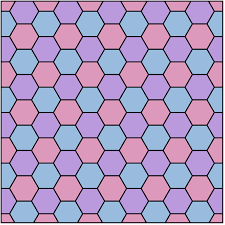
\includegraphics [scale=0.5] {image/pavage_hexagonal.png}
    \caption{Exemple de pavage régulier avec des hexagones}
\end{figure}



\newpage

\subsection{Pavage périodique / aperiodique}

Une des applications scientifique du pavage est dans la cristallographie \footnote{La cristallographie est une science qui étudie la structure atomique des cristaux et des minéraux pour modéliser des arrangements périodiques d'atomes}. On remarque des structures périodiques dans l'empilement des atomes dans les cristaux.

\hspace{1.5cm}

\textbf{\textsc{Périodique}}

Un pavage $P=\left \{ p_{k}\subset \mathbb{R}^{2} \right \}_{1\leq k\leq n}$ est périodique s'il est composé de sous-espace images l'un de l'autre par translation sur une grille régulière.

\begin{figure} [h]
    \center
    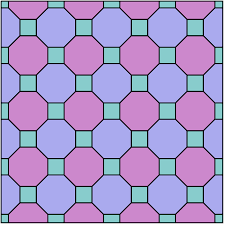
\includegraphics [scale=0.3] {image/pavage_périodique_irrégulier.png}
    \caption{Exemple de pavage irrégulier périodique}
\end{figure}

On peut le retrouver sur les murs du palais de l'Alhambra ou sur les dessins de \nameref{M.C Escher}.
Ce type de pavage est connu depuis l’antiquité comme motif décoratif.

\begin{figure} [h]
    \center
    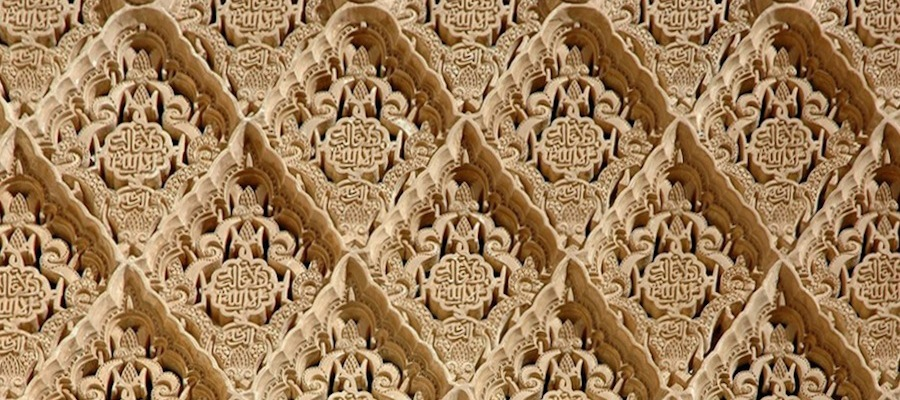
\includegraphics [scale=0.3] {image/Alhambra.jpg}
    \caption{Portion de mur de l'Alhambra}
\end{figure}

Le mathematicien russe \nameref{Fedorov} a montré que seulement 17 types de pavages periodiques existaient dans le plan.
Deux pavages sont considérés de meme type s’ils sont invariant par le même groupe d’isométrie.
On retrouve les 17 types de pavages à l'Alhambra.

\newpage

\hspace{1.5cm}

\textbf{\textsc{Apériodique}}

Un pavage est apériodique s'il n'est pas composé d'ensemble d'élements répétés périodiquement sur une grille régulière. Un puzzle est un pavage apériodique, la forme est unique pour chaque pièce et les couleurs ne représentent pas de motifs périodiques.

\hspace{1cm}

Le pavage de \nameref{Penrose} est l'exemple le plus connu.
Les 17 pavages périodiques du plan étant déjà connus, Penrose décida de s'interesser aux pavages apériodiques par divertissement mathématique. Ce n'est que 10 ans aprés son premier article publié en 1974 présentant des pavages apériodiques, qu'il a été découvert des matériaux présentants des structures ordonnées mais non périodiques : les quasi-cristaux.
Ce type de pavage est quasi-périodiques puisque tout motif apparaissant dans le pavage réapparait régulièrement mais apériodiquement.

\hspace{1.5cm}


Il existe 4 pavages de Penrose différents, chacun ayant une infinité de variantes :

\hspace{1cm}

- Pentagonal ( avec des pentagones, losanges, pentagrammes et des portions de pentagramme).

\begin{figure} [h]
    \center
    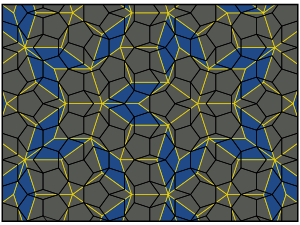
\includegraphics [scale=0.4] {image/penrose_pentagone.png}
    \caption{Pavage de Penrose pentagonal tracé en noir}
\end{figure}

Il est le premier découvert par Penrose. Le plan n'est pas recouvable par des pentagones mais des losanges fins, pentagrammes et des "bateaux" comblent les interstices tout en gardant l'ordre apériodique.

\clearpage

- Cerfs-volant et fléchettes ( avec deux quadrilatères, l'un convexe, l'autre concave \footnote{Un polygone est convexe si tous ses angles intérieurs sont inférieurs à 180°, il est concave si au moins un angle intérieur est supérieur à 180°} ).

\begin{figure} [h]
    \center
    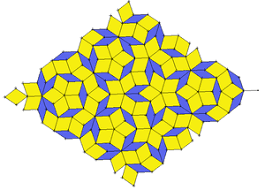
\includegraphics [scale=0.5] {image/penrose_flechette.png}
    \caption{Pavage de Penrose en fléchettes, ici, le quadrilatère bleu est convexe et le jaune concave}
\end{figure}

- Losanges ( avec deux sortes de losanges, fins et gros )

\begin{figure} [h]
    \center
    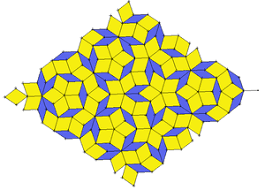
\includegraphics [scale=0.5] {image/penrose_losange.png}
    \caption{Pavage de Penrose avec des losanges}
\end{figure}

- Triangle d’or ( avec des triangles isocèles dont les cotés ont des longueurs proportionnelles au nombre d’or )

\begin{figure} [h]
    \center
    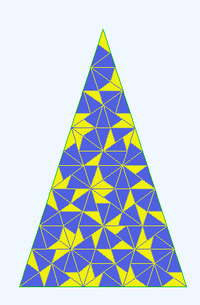
\includegraphics [scale=0.5] {image/penrose_tri.png}
    \caption{Pavage de Penrose avec de triangles d'or, la base}
\end{figure}

\newpage

\section{Pavage du plan par des dominos}

Aucun algorithme ne dit systématiquement si n'importe quelle portion de plan est pavable par des polygones.
On dit que le problème est indécidable \footnote{Problème qui ne peut pas être résolu algorithmiquement en un temps toujours fini.}.

Dans cette partie, nous allons alors nous concentrer sur le pavage par dominos $2*1$ et $1*2$ dans le plan euclidien.
Soit  $P=\left \{ p_{k}\subset \mathbb{Z}^{2} \right \}_{1\leq k\leq n}$ un pavage avec $p_{k}$ les n dominos. P est une portion finie de plan euclidien délimitée par des côtés de longueur entière parallèles aux axes du plan euclidien.
On considere aussi que ce sous-espace de $\mathbb{Z}^{2}$ n’a pas de trous. Ce type de pavage est régulier par isométrie du plan et quasi-périodique.
Les dominos ne doivent pas se chevaucher et sont connexes à au moins un autre domino.

\begin{figure} [h]
    \center
    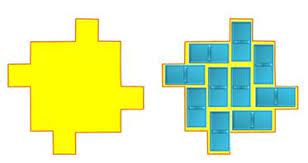
\includegraphics [scale=0.5] {image/pavage_domino.jpg}
    \caption{Exemple d'un pavage possible d'une portion du plan par des dominos }
\end{figure}



\subsection{Polyomino}

Un polyomino est une réunion connexe et finis de carrés unitaires de $\mathbb{Z}^{2}$ (ex: formes de Tetris) chaque carré a au moins un coté connexe à un autre.
Il existe 2 groupes de polyomino : à forme fixée et à forme libre (qui peut subir une rotation ).

\begin{figure} [!h]
    \center
    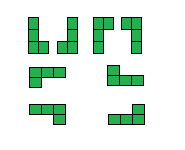
\includegraphics [scale=0.5] {image/polyomino_libre.png}
    \caption{8 formes fixes pour une même forme libre d'un tétromino (4 carrés)}
\end{figure}

\clearpage

\hspace{1cm}

Un domino est un polyomino composé de 2 carrés. Il n’a qu’une forme libre possible et deux formes fixées : $2*1$ et $1*2$.
Un triomino est composé de 3 carrés et a deux formes libres possibles.

\hspace{1cm}

\begin{figure} [!h]
    \center
    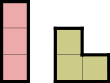
\includegraphics [scale=0.5] {image/triomino.png}
    \caption{Les deux formes libres du triomino}
\end{figure}

\hspace{1cm}

Ainsi de suite, un decamino (10 carrés) a 4655 formes libres différentes.

Un pavage dans $\mathbb{Z}^{2}$ est un polyomino composé de sous-polyominos (ici les dominos).
Etant donné un ensemble finis de polyomino, la pavabilité est décidable puisqu'on peut toujours essayer toutes les combinaisons possibles.
Il s'agit alors de trouver un algorithme efficace pour dire si un polyomino est pavable ou non par des dominos.

\newpage

\subsection{Algorithme de \nameref{Thurston}}

L'algorithme de Thurston décide en temps linéaire si un polyomino sans trou est pavable par dominos et le construit si oui.
Prenons un polyomino de n cases, sa complexité est en $O\left ( nlog\left ( n \right ) \right )$. Soit p son périmetre, p=racine de n car n est son air.
Ainsi on peut aussi dire que sa complexité est en $O\left ( p^{2}log\left ( p^{2} \right ) \right )$.

Considérons un polyomino sans trou. On colorie ses cases comme un damier (cadrié en noir et blanc). Ce polyomino peut etre représenté par un graphe dont les arrètes seraient les cotés des cases du damier.
On definit une fonction de hauteur h appliqué aux n sommets du graphe G {v0,v1,...,vn}.
Partons d'un sommet v0 quelconque.

- $h\left ( v_{0} \right )= 0$

Soient vi et vj deux sommets de G reliés par une arrete alors

- $h\left ( v_{j} \right )= h\left ( v_{i} \right ) + 1$ si l'arrete (vi,vj) a sur sa gauche une case noire.

- $h\left ( v_{j} \right )= h\left ( v_{i} \right ) - 1$ si non.




\newpage

\subsection{Nombre de pavage dans un polyomino}

\hspace{1cm}

Il existe des formules mathématiques pour calculer le nombre de pavage possible de polyominos particuliers. Nous allons voir que le nombre de pavage augmente trés rapidement en fonction du nombre de cases.

\hspace{1cm}

\subsubsection{Nombre de pavage dans un rectangle mxn}

\hspace{1.5cm}

\textbf{\textsc{2xn}}

Soit $f_{n}$ le nombre de pavage possible.

Le premier cas est le rectangle $2*1$, il y a bien sûr qu’un pavage possible : $f_{1} = 1$.

Le deuxieme cas est un rectangle $2*2$, où deux pavages sont possibles deux dominos en long ou deux dominos en large.

\begin{figure} [!h]
    \center
    \includegraphics [scale=0.5] {image/pavage_carré.png}
    \caption{Les deux facons de paver un carré  $2*2$}
\end{figure}

Dans un cas général, si on ajoute au rectangle $2*n$ un rectangle sur le coté de longueur 2, le nombre $f_{n}$ de pavage augmente de 1.

\begin{figure} [!h]
    \center
    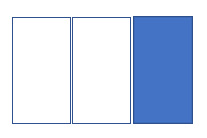
\includegraphics [scale=0.5] {image/domino_n+1.png}
    \caption{Ajout d'un domino depuis le rectangle $2*2$}
\end{figure}

Mais on peut aussi ajouter deux rectangles en long au rectangle $2*(n+1)$ sur le coté de longueur 2. Dans ce cas là, le nombre $f_{n-1}$ de pavage augmente de 2.

\begin{figure} [!h]
    \center
    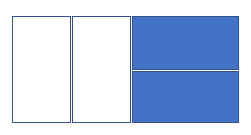
\includegraphics [scale=0.5] {image/domino_n+2.png}
    \caption{Ajout de deux dominos depuis le rectangle $2*2$}
\end{figure}

Ainsi on a tous les pavages du rectangle $2*(n+1)$ et $f_{n+1} = f_{n} + f_{n-1}$.

Ce sont les nombres de Fibonacci : 1, 2, 3, 5, 8, 13, 21, 34, 55…

Le rectangle de dimension $2*10$ a 89 pavages possibles.

\hspace{1.5cm}

\textbf{\textsc{3x2n}}

Bien sûr un rectangle de dimension $3*(2n+1)$ est impossible à paver par des dominos puisqu'il y a un nombre impair de cases.

Le premier cas est un rectangle $3*2$, il y a trois pavages possibles, $f_{3} = 3$.

\begin{figure} [!h]
    \center
    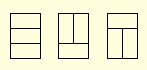
\includegraphics [scale=0.7] {image/pavage_3x2.png}
    \caption{Les 3 pavages possibles du rectangle $3*2$}
\end{figure}

Si on y ajoute un deuxieme blos $3*2$, il y a $3*3$ pavages possibles dans chaque bloc.
Mais on peut aussi former 2 pavages dans le rectangle $3*4$ sans former de bloc $3*2$.

\begin{figure} [!h]
    \center
    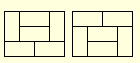
\includegraphics [scale=0.7] {image/pavage_3x6.png}
    \caption{Les 2 pavages avec un rectangle $3*4$}
\end{figure}

Ainsi, en général, si on appelle $a_{n}$ le nombre de pavage dans un rectangle de $3*2n$, $a_{n+1}$ est obtenu en y ajoutant un bloc de 3×2.
Ce qui donne $3*a_{n}$, plus toutes les combinaisons où ce bloc est concaténé avec des blocs précédents sans former de blocs de 3×2.
Dans ce cas, il y a un bloc de $3*2i$ suivi d'un bloc de $3*2j$ sans blocs internes. Il n'y a que deux possibilités obtenues en dupliquant les dominos bleus de l'exemple ci dessous.

\begin{figure} [!h]
    \center
    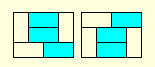
\includegraphics [scale=0.7] {image/pavage-3x6_bleu.png}
\end{figure}

Chacune de ces possibilités donne donc lieu à $a_{i}*2$ possibilités.
Donc $a_{n+1} = 3*a_{n} + 2\sum_{i}^{n}a_{i}$

\hspace{1cm}

Calculons $a_{n+1} - a_{n}$
\\$a_{n+1} - a_{n}   = 3*a_{n} + 2\sum_{i}^{n}a_{i} - 3*an-1 - 2\sum_{i}^{n-1}a_{i}$


$= 3*a_{n} - a_{n-1} + 2\sum_{i}^{n-1}a_{i} - 2\sum_{i}^{n-1}a_{i}$


$= 3*a_{n} - a_{n-1}$ \\et finalement $a_{n+1} = 4*a_{n} - a_{n-1}$

    \hspace{1cm}

    \noindent$a_{1} = 3$
    \\$a_{2} = 4*3 - 1 = 11$
\\$a_{3} = 4*11 - 3 = 41$
    \\$a_{10} = 4*a_{9} - a_{8} = 413403$ ...


\hspace{2cm}

\textbf{\textsc{mxn}}

Le cas géneral est beaucoup plus compliqué à demontrer mais voici la formule qui permet de trouver le nombre de pavage possible dans un rectangle mxn:

\begin{center}
    $\prod_{j=1}^{\left \lceil \frac{m}{2} \right \rceil} \prod_{k=1}^{\left \lceil \frac{n}{2} \right \rceil}\left ( 4\cos^{2}\frac{j\pi }{m+1}+4\cos^{2}\frac{k\pi }{n+1} \right )$
\end{center}

Il est étonnant de se dire que le résultat de cette formule est toujours positif.

Essayons pour un rectangle $2*4$ : $\prod_{j=1}^{\left \lceil \frac{2}{2} \right \rceil} \prod_{k=1}^{\left \lceil \frac{4}{2} \right \rceil}\left ( 4\cos^{2}\frac{j\pi }{2+1}+4\cos^{2}\frac{k\pi }{4+1} \right )$

%Essayons pour un rectangle $5*7$ : $\prod_{j=1}^{\left \lceil \frac{5}{2} \right \rceil} \prod_{k=1}^{\left \lceil \frac{7}{2} \right \rceil}\left ( 4\cos^{2}\frac{j\pi }{5+1}+4\cos^{2}\frac{k\pi }{7+1} \right )$



\hspace{2cm}

\subsubsection{Nombre de pavage dans un diamant aztèque}

Un diamant aztèque est un polyomino toujours pavable par des dominos.

\hspace{1cm}

\begin{figure} [!h]
    \center
    \includegraphics [scale=0.5] {image/diamants_aztèques.png}
    \caption{Diamants aztèques d'ordre 1, 2, 3 et 6}
\end{figure}

\hspace{1cm}

Il n'y a que deux facons de paver un diamant d'ordre 1 (voir figure 11).

Il y a 8 pavages pour un diamant d'ordre 2.

\hspace{2cm}

\begin{figure} [!h]
    \center
    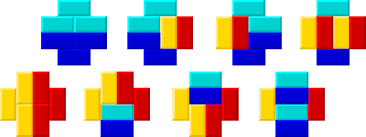
\includegraphics [scale=0.5] {image/diamant_2.png}
    \caption{Diamants azteques d'ordre 2}
\end{figure}

\hspace{1cm}

Le nombre de pavage possible dans un diamant aztèque d'ordre n est calculable depuis la formule que nous allons pas démontrer :

\begin{center}
    $f_{n}=2^{\frac{n\left ( n+1 \right )}{2}}$
\end{center}

\clearpage

\section{Description de notre projet}

Nous avons codé en C un programme informatique qui prend en paramètre un ensemble de direction (Nord (N), Sud (S), Est (E), et Ouest (O)) et qui affiche avec SDL, si c'est possible, un pavage de la forme rentrée par l'utilisateur.



\subsection{M.C Escher}

\clearpage

\section{Références}

\subsection{M.C Escher}

\label{M.C Escher}

Artiste neerlandais né en 1898 et mort en 1972 très sensible à l’art islamique géométrique et aux mathématiques, il a beaucoup travaillé sur le thème des pavages.

\begin{figure} [!h]
    \center
    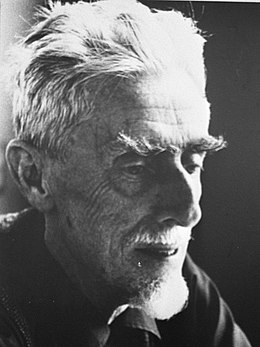
\includegraphics [scale=0.25] {image/escher.jpg}
    \caption{Portrait d'Escher en 1971, 1 an avant son décès}
\end{figure}

\begin{figure} [!h]
    \center
    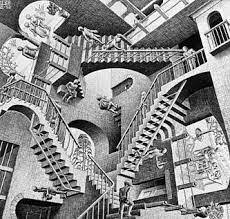
\includegraphics [scale=0.4] {image/dessin1_escherjpg.jpg}
    \caption{Célèbre dessin impossible d'Escher}
\end{figure}

\begin{figure} [!h]
    \center
    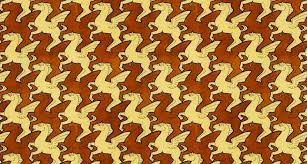
\includegraphics [scale=0.4] {image/dessin2_escherjpg.jpg}
    \caption{Dessin d'un pavage régulier périodique, M.C Escher}
\end{figure}

\begin{figure} [!h]
    \center
    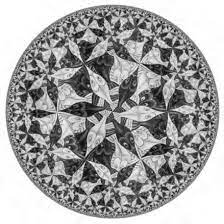
\includegraphics [scale=0.4] {image/dessin3_escher.jpg}
    \caption{Dessin d'un pavage périodique dans un plan hyperbolique}
\end{figure}

\newpage

\subsection{Thurston}

\label{Thurston}

William Thurston est un mathématicien américain né en 1946 et mort en 2012, spécialisé dans la topologie sur les espaces bi et tri-dimensionnels et dont il fut recompenser par la médaille Fields en 1983.

\begin{figure} [!h]
    \center
    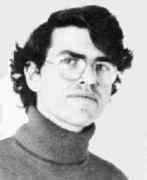
\includegraphics [scale=0.5] {image/thurston.jpg}
    \caption{Portrait de Thurston en 1991}
\end{figure}

\newpage

\subsection{Fedorov}

\label{Fedorov}

Evgraf Fedorov est un mathématicien cristallographe russe né en 1853 et mort en 1919 (polytope à developper)

\begin{figure} [!h]
    \center
    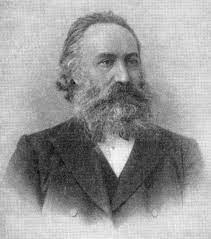
\includegraphics [scale=0.5] {image/Fedorov.jpg}
    \caption{Portrait d'Evgraf Fedorov à la fin du 19eme siècle}
\end{figure}

\newpage

\subsection{Penrose}

\label{Penrose}

Roger Penrose est un mathématicien, astrophysicien et philosophe des sciences britannique né en 1931. Il a travaillé avec le célèbre physicien Stephen Hawking sur la théorie de l'origine de l'univers et la théorie de l'effondrement des étoiles sur elles-mêmes.
Il travailla aussi sur les pavages apériodiques et sur des objets impossibles tels que le triangle de Penrose.

\begin{figure} [!h]
    \center
    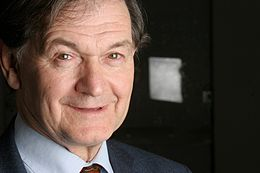
\includegraphics [scale=0.5] {image/Penrose.jpg}
    \caption{Portrait de Roger Penrose 2005}
\end{figure}

\begin{figure} [!h]
    \center
    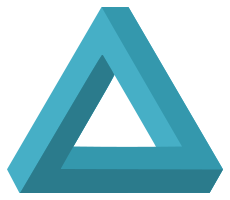
\includegraphics [scale=0.5] {image/tri_penrose.png}
    \caption{Triangle de Penrose}
\end{figure}

%\nocite{*}
%\bibliographystyle{plain}
%\bibliography{biblio} % fichier biblio.bib
\end{document}

